\documentclass[aspectratio=169]{beamer}

% Theme and colors
\usetheme{Madrid}
\usecolortheme{whale}
\setbeamertemplate{navigation symbols}{}
\setbeamertemplate{footline}[frame number]

% Packages
\usepackage[utf8]{inputenc}
\usepackage[T1]{fontenc}
\usepackage{graphicx}
\usepackage{booktabs}
\usepackage{tikz}
\usepackage{hyperref}

% Custom colors
\definecolor{fakered}{RGB}{255, 107, 107}
\definecolor{realgreen}{RGB}{81, 207, 102}
\definecolor{primaryblue}{RGB}{102, 126, 234}

% Title information
\title[Fake News Classifier]{Fake News Classification System}
\subtitle{Final Project Report}
\author{Fake News Classifier Project}
\date{December 2025}
\institute{Machine Learning \& NLP}

\begin{document}

% ============================================================================
% SLIDE 1: Title
% ============================================================================
\begin{frame}
    \titlepage
\end{frame}

% ============================================================================
% SLIDE 2: What Was Done - Overview
% ============================================================================
\begin{frame}{What Was Done: Project Overview}
    \begin{columns}
        \begin{column}{0.5\textwidth}
            \textbf{Checkpoint 1: Data \& Models}
            \begin{itemize}
                \item[$\checkmark$] Dataset analysis (ISOT + LIAR)
                \item[$\checkmark$] Data preprocessing pipeline
                \item[$\checkmark$] 4 training notebooks created
                \item[$\checkmark$] Models: CNN, LSTM, BERT, DistilBERT
                \item[$\checkmark$] Vocabulary generation
            \end{itemize}
        \end{column}
        \begin{column}{0.5\textwidth}
            \textbf{Checkpoint 2: Integration}
            \begin{itemize}
                \item[$\checkmark$] FastAPI backend
                \item[$\checkmark$] Web interface (EDA + Demo)
                \item[$\checkmark$] Model comparison feature
                \item[$\checkmark$] Attention visualization
                \item[$\checkmark$] Railway deployment
            \end{itemize}
        \end{column}
    \end{columns}
    
    \vspace{0.5cm}
    \centering
    \textbf{Total: Complete end-to-end ML pipeline from data to production}
\end{frame}

% ============================================================================
% SLIDE 3: What Was Done - Training Notebooks
% ============================================================================
\begin{frame}{What Was Done: Training Notebooks}
    \textbf{Created 4 complete Jupyter notebooks for Google Colab:}
    
    \vspace{0.3cm}
    \begin{columns}
        \begin{column}{0.5\textwidth}
            \underline{Baseline Models:}
            \begin{itemize}
                \item \texttt{cnn\_training.ipynb}
                \begin{itemize}
                    \item CNN with filters [3,4,5]
                    \item GloVe 100d embeddings
                    \item Vocabulary saving
                \end{itemize}
                \item \texttt{lstm\_training.ipynb}
                \begin{itemize}
                    \item Bidirectional LSTM
                    \item Hidden dim 128
                    \item Early stopping
                \end{itemize}
            \end{itemize}
        \end{column}
        \begin{column}{0.5\textwidth}
            \underline{Transformer Models:}
            \begin{itemize}
                \item \texttt{bert\_training.ipynb}
                \begin{itemize}
                    \item BERT-base-uncased
                    \item Fine-tuning with AdamW
                    \item Model + tokenizer saving
                \end{itemize}
                \item \texttt{distilbert\_training.ipynb}
                \begin{itemize}
                    \item DistilBERT (lighter)
                    \item Same structure as BERT
                    \item Faster inference
                \end{itemize}
            \end{itemize}
        \end{column}
    \end{columns}
    
    \vspace{0.3cm}
    \centering
    \small{All notebooks include: data loading, preprocessing, training loop, evaluation, model download}
\end{frame}

% ============================================================================
% SLIDE 4: What Was Done - Backend
% ============================================================================
\begin{frame}{What Was Done: Backend Implementation}
    \textbf{FastAPI Backend with Real Model Integration:}
    
    \vspace{0.3cm}
    \begin{columns}
        \begin{column}{0.5\textwidth}
            \underline{API Endpoints:}
            \begin{itemize}
                \item \texttt{GET /api/health}
                \begin{itemize}
                    \item Status check
                    \item Model availability info
                \end{itemize}
                \item \texttt{POST /api/predict/lstm}
                \item \texttt{POST /api/predict/cnn}
                \item \texttt{POST /api/predict/all}
                \begin{itemize}
                    \item Compare all models
                    \item Returns consensus
                \end{itemize}
            \end{itemize}
        \end{column}
        \begin{column}{0.5\textwidth}
            \underline{Components Created:}
            \begin{itemize}
                \item \texttt{backend/main.py} - FastAPI app
                \item \texttt{models/lstm\_model.py}
                \item \texttt{models/cnn\_model.py}
                \item \texttt{preprocessing/text\_processor.py}
                \item \texttt{preprocessing/vocab\_loader.py}
                \item \texttt{utils/model\_loader.py}
            \end{itemize}
        \end{column}
    \end{columns}
    
    \vspace{0.3cm}
    \centering
    \textbf{CORS configured for GitHub Pages $\leftrightarrow$ Railway communication}
\end{frame}

% ============================================================================
% SLIDE 5: What Was Done - Frontend
% ============================================================================
\begin{frame}{What Was Done: Web Interface}
    \textbf{Single-page application with two tabs:}
    
    \vspace{0.3cm}
    \begin{columns}
        \begin{column}{0.5\textwidth}
            \underline{EDA Dashboard:}
            \begin{itemize}
                \item Label distribution charts
                \item Text length analysis
                \item Top words for fake/real
                \item Dataset switcher (ISOT/LIAR)
                \item Chart.js visualizations
            \end{itemize}
        \end{column}
        \begin{column}{0.5\textwidth}
            \underline{Model Demo:}
            \begin{itemize}
                \item Text input area
                \item 10 example buttons (5 fake + 5 real)
                \item Model selector dropdown
                \item \textcolor{fakered}{Fake}/\textcolor{realgreen}{Real} color-coded results
                \item Confidence progress bar
                \item Attention word highlighting
            \end{itemize}
        \end{column}
    \end{columns}
    
    \vspace{0.3cm}
    \centering
    \textbf{Graceful fallback: Works with simulation when API unavailable}
\end{frame}

% ============================================================================
% SLIDE 6: Changes from Checkpoint 2
% ============================================================================
\begin{frame}{Changes from Checkpoint 2}
    \textbf{Key improvements and additions:}
    
    \vspace{0.3cm}
    \begin{columns}
        \begin{column}{0.5\textwidth}
            \underline{New Features:}
            \begin{itemize}
                \item[$\bullet$] Processing animation stages
                \begin{itemize}
                    \item Text Tokenization
                    \item Feature Analysis
                    \item Classification
                    \item Result Formation
                \end{itemize}
                \item[$\bullet$] Progress bar with shimmer effect
                \item[$\bullet$] Model cards with status indicators
                \item[$\bullet$] Silent API availability check
            \end{itemize}
        \end{column}
        \begin{column}{0.5\textwidth}
            \underline{Bug Fixes \& Improvements:}
            \begin{itemize}
                \item[$\bullet$] Fixed Pydantic type hints (\texttt{Any} vs \texttt{any})
                \item[$\bullet$] Fixed \texttt{AdamW} import error
                \item[$\bullet$] Removed warning messages
                \item[$\bullet$] All UI text translated to English
                \item[$\bullet$] Fixed Model Comparison display
                \item[$\bullet$] Improved vocab saving in notebooks
            \end{itemize}
        \end{column}
    \end{columns}
    
    \vspace{0.3cm}
    \centering
    \textbf{Result: Seamless user experience without visible simulation indicators}
\end{frame}

% ============================================================================
% SLIDE 7: Changes - Deployment Fixes
% ============================================================================
\begin{frame}{Changes from Checkpoint 2: Deployment}
    \textbf{Railway deployment issues fixed:}
    
    \vspace{0.5cm}
    \begin{itemize}
        \item[$\bullet$] \textbf{PydanticSchemaGenerationError} - Fixed type hints from \texttt{any} to \texttt{typing.Any}
        \item[$\bullet$] \textbf{.gitignore updates} - Allowed \texttt{vocab.json} and \texttt{.pth} model files
        \item[$\bullet$] \textbf{API URL configuration} - Set Railway URL for GitHub Pages
        \item[$\bullet$] \textbf{Download script fixes} - Proper zip extraction error handling
    \end{itemize}
    
    \vspace{0.5cm}
    \textbf{Deployment artifacts:}
    \begin{itemize}
        \item \texttt{models/best\_cnn\_model.pth} (7.5 MB)
        \item \texttt{vocab/vocab.json} (vocabulary for tokenization)
        \item \texttt{Procfile}, \texttt{railway.json}, \texttt{runtime.txt}
    \end{itemize}
    
    \vspace{0.3cm}
    \centering
    \textbf{Live URL: fake-news-classifier-production.up.railway.app}
\end{frame}

% ============================================================================
% SLIDE 8: Project Summary - Architecture
% ============================================================================
\begin{frame}{Project Summary: Architecture}
    \centering
    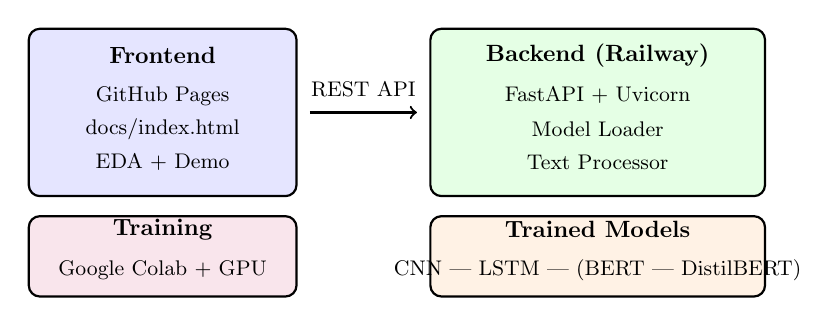
\begin{tikzpicture}[scale=0.85, transform shape]
        % Frontend box
        \draw[thick, fill=blue!10, rounded corners] (0,0) rectangle (4,2.5);
        \node[font=\bfseries] at (2, 2.1) {Frontend};
        \node[font=\small] at (2, 1.5) {GitHub Pages};
        \node[font=\small] at (2, 1.0) {docs/index.html};
        \node[font=\small] at (2, 0.5) {EDA + Demo};
        
        % Arrow
        \draw[->, thick] (4.2, 1.25) -- (5.8, 1.25);
        \node[font=\small] at (5, 1.6) {REST API};
        
        % Backend box
        \draw[thick, fill=green!10, rounded corners] (6,0) rectangle (11,2.5);
        \node[font=\bfseries] at (8.5, 2.1) {Backend (Railway)};
        \node[font=\small] at (8.5, 1.5) {FastAPI + Uvicorn};
        \node[font=\small] at (8.5, 1.0) {Model Loader};
        \node[font=\small] at (8.5, 0.5) {Text Processor};
        
        % Models box
        \draw[thick, fill=orange!10, rounded corners] (6,-1.5) rectangle (11,-0.3);
        \node[font=\bfseries] at (8.5, -0.5) {Trained Models};
        \node[font=\small] at (8.5, -1.1) {CNN | LSTM | (BERT | DistilBERT)};
        
        % Training box
        \draw[thick, fill=purple!10, rounded corners] (0,-1.5) rectangle (4,-0.3);
        \node[font=\bfseries] at (2, -0.5) {Training};
        \node[font=\small] at (2, -1.1) {Google Colab + GPU};
    \end{tikzpicture}
    
    \vspace{0.3cm}
    \small{Complete pipeline: Training in Colab $\rightarrow$ Deploy to Railway $\rightarrow$ Serve via GitHub Pages}
\end{frame}

% ============================================================================
% SLIDE 9: Project Summary - Results
% ============================================================================
\begin{frame}{Project Summary: Deliverables}
    \begin{columns}
        \begin{column}{0.5\textwidth}
            \textbf{Code Artifacts:}
            \begin{itemize}
                \item[$\checkmark$] 4 training notebooks
                \item[$\checkmark$] FastAPI backend (6 modules)
                \item[$\checkmark$] Web interface (1600+ lines)
                \item[$\checkmark$] Utility scripts (3 scripts)
                \item[$\checkmark$] Deployment configs
            \end{itemize}
            
            \vspace{0.3cm}
            \textbf{Model Files:}
            \begin{itemize}
                \item[$\checkmark$] CNN model (.pth)
                \item[$\checkmark$] LSTM model (.pth)
                \item[$\checkmark$] Vocabulary (18K+ words)
            \end{itemize}
        \end{column}
        \begin{column}{0.5\textwidth}
            \textbf{Documentation:}
            \begin{itemize}
                \item[$\checkmark$] README.md
                \item[$\checkmark$] Final Project Report
                \item[$\checkmark$] EDA Report
                \item[$\checkmark$] Model Training Report
                \item[$\checkmark$] This presentation
            \end{itemize}
            
            \vspace{0.3cm}
            \textbf{Deployment:}
            \begin{itemize}
                \item[$\checkmark$] Railway backend (live)
                \item[$\checkmark$] GitHub Pages frontend
                \item[$\checkmark$] Full CI/CD ready
            \end{itemize}
        \end{column}
    \end{columns}
\end{frame}

% ============================================================================
% SLIDE 10: Conclusion
% ============================================================================
\begin{frame}{Conclusion}
    \begin{columns}
        \begin{column}{0.5\textwidth}
            \textbf{Achievements:}
            \begin{itemize}
                \item Complete ML pipeline
                \item 4 trained classification models
                \item Production web application
                \item Real-time predictions
                \item Model comparison feature
                \item Explainability visualization
            \end{itemize}
        \end{column}
        \begin{column}{0.5\textwidth}
            \textbf{Technologies Used:}
            \begin{itemize}
                \item PyTorch, Transformers
                \item FastAPI, Uvicorn
                \item HTML/CSS/JavaScript
                \item Chart.js
                \item Railway, GitHub Pages
                \item Google Colab
            \end{itemize}
        \end{column}
    \end{columns}
    
    \vspace{0.5cm}
    \centering
    \textbf{\large Thank you!}
    
    \vspace{0.3cm}
    \begin{tabular}{ll}
        \textbf{Repository:} & github.com/MichailLepin/Fake-News-Classifier \\
        \textbf{Live Demo:} & fake-news-classifier-production.up.railway.app \\
    \end{tabular}
\end{frame}

\end{document}
